\documentclass[11pt]{article}

% --- Style: arxiv.sty (as specified) ---
\usepackage{arxiv}

% --- Core packages ---
\usepackage[utf8]{inputenc}
\usepackage[T1]{fontenc}
\usepackage{amsmath,amssymb,amsfonts}
\usepackage{graphicx}
\usepackage{booktabs}
\usepackage{multirow}
\usepackage{hyperref}
\usepackage[capitalize]{cleveref}
\usepackage{xcolor}

% --- Custom commands ---
\newcommand{\eps}{\varepsilon}
\newcommand{\todo}[1]{\textcolor{red}{[TODO: #1]}}

\title{Hybrid Quantum-Classical Traffic Sign Recognition:\\
An Adversarial Robustness Study on GTSRB}

\author{%
  Leyu Fu\\
  Beijing JiaoTong University\\
  \texttt{leyufu@bjtu.edu.cn}\\
}

\undertitle{A Preprint}
\headeright{A Preprint}
\date{\today}

\begin{document}
\maketitle

\begin{abstract}
Traffic sign recognition is a safety-critical component of autonomous driving
visual perception, yet deep classifiers remain vulnerable to adversarial
perturbations. While quantum-classical hybrid neural networks have been
explored on small-scale vision benchmarks, their adversarial robustness on
safety-critical, real-world tasks has not been systematically evaluated under
a fair comparison with a strong classical baseline. In this work we present,
to the best of our knowledge, the first such study on the German Traffic
Sign Recognition Benchmark (GTSRB, 43 classes). We compare four WideResNet
variants that share an identical convolutional backbone (WRN-28-4) and
achieve near-identical clean accuracy within a 0.7 percentage-point margin
(98.73\%--99.40\%): a strong classical classifier, a hybrid model with an
8-qubit variational quantum layer, and two structural ablations that remove
or replace the quantum layer. Under white-box digital attacks (FGSM, PGD,
and a Carlini--Wagner-style $L_\infty$ variant), the hybrid quantum model
exhibits consistently higher robust accuracy. At $\eps = 8/255$ under PGD,
it retains 26.15\% accuracy versus 15.0\% for the strong classical baseline.
Crucially, the two ablations recover the classical baseline's
behavior (14.8\% and 13.8\%), isolating the robustness gain to the quantum
layer itself rather than the 8-dimensional bottleneck or an additional
nonlinear head. Our evaluation uses a pixel-space attack protocol with a
\texttt{NormalizeWrapper}, ensuring that $\eps = k/255$ retains its
physical meaning. We discuss possible mechanisms, the limitations of
single-seed evaluation and simulator-based quantum circuits, and the
implications for deploying quantum-augmented models in safety-critical
perception pipelines.
\keywords{Quantum machine learning \and Adversarial robustness \and
Traffic sign recognition \and Autonomous driving \and Hybrid quantum-classical networks}
\end{abstract}

%======================================================================
\section{Introduction}
\label{sec:intro}
%======================================================================

% --- 1.a Trends ---
Deep neural networks have become the backbone of modern autonomous driving
visual perception, powering traffic sign recognition, object detection, and
lane estimation~\cite{bojarski2016nvidia,grigorescu2020autonomous_survey}.
Their accuracy on standard benchmarks is now near-saturated: the German
Traffic Sign Recognition Benchmark (GTSRB)~\cite{stallkamp2012gtsrb} is
routinely solved above 99\% test accuracy. This performance, however,
masks a fragility that is unacceptable in safety-critical settings.

% --- 1.b Valueness ---
Traffic sign misclassification can cause catastrophic failure of downstream
planning and control. A stop sign read as a speed-limit sign, or a
yield sign erased by a small visual perturbation, translates directly into
hazardous behavior. Adversarial examples---imperceptible or physically
realizable perturbations crafted to flip a model's prediction---are therefore
not merely an academic concern but a concrete threat to autonomous driving
safety~\cite{eykholt2018rp2,chen2018shapeshifter}.

% --- 1.c Existing Problem ---
The adversarial robustness of deep classifiers has been studied extensively,
yet two gaps remain. First, the vast majority of quantum machine learning
(QML) robustness studies are confined to small toy benchmarks (MNIST,
CIFAR-10), and---when they compare to classical baselines at all---do so
against weak or capacity-mismatched models. Second, the existing autonomous
driving adversarial literature is almost entirely classical; the behavior of
\emph{quantum-augmented} classifiers under attack in this domain is unknown.

% --- 1.d Research issues ---
Approaches to adversarial robustness can be grouped into two lines.

\textbf{Group A: Classical robustness in autonomous driving vision.}
A large body of work characterizes attacks on, and defenses for, classical
traffic sign and traffic light classifiers, including the Robust Physical
Perturbations (RP2) attack on stop signs~\cite{eykholt2018rp2}, the
ShapeShifter targeted attack on Faster R-CNN detectors~\cite{chen2018shapeshifter},
and the adversarial patch paradigm~\cite{brown2017adversarialpatch}. On the
defense side, adversarial training~\cite{madry2018pgd} and certified
methods have been proposed. \emph{Limitation}: these works treat the
classifier as a fixed classical component and do not consider whether
alternative computational substrates---such as variational quantum
circuits---alter the adversarial landscape.

\textbf{Group B: Quantum machine learning robustness.}
Variational quantum circuits have been proposed as trainable layers within
hybrid quantum-classical networks~\cite{farhi2018quantum,schuld2014quantum,benedetti2019hybrid},
including quantum convolutional architectures~\cite{cong2019qcnn,herrera2019qcnn_vision}.
A smaller line investigates their adversarial
properties~\cite{lu2020quantum_adv,weber2020robust,preset2022qmlrobust}.
\emph{Limitation}: these studies (i) evaluate on low-resolution toy tasks,
(ii) compare against classical baselines that are either shallow or
deliberately bottlenecked to match a quantum dimension, and (iii) do not
address safety-critical perception. Consequently, it remains open whether
a quantum layer provides robustness beyond what a comparably accurate
strong classical model already offers.

% --- 1.d.5 Contributions & RQs ---
This paper closes that gap. We study a quantum-classical hybrid WideResNet
on GTSRB under white-box digital attacks, compared against a \emph{strong}
classical WideResNet baseline with no artificial bottleneck, and further
isolate the quantum contribution through two structural ablations. We pose
two research questions:

\begin{description}
  \item[\textbf{RQ1}.] On a safety-critical traffic sign task, does a
    hybrid quantum-classical classifier exhibit adversarial robustness
    beyond a strong classical baseline of comparable clean accuracy?
  \item[\textbf{RQ2}.] If such a difference exists, is it attributable to the
    quantum layer itself, or to confounds---the low-dimensional bottleneck
    or an additional nonlinear head---that the quantum layer introduces?
\end{description}

Our contributions are as follows.
\begin{enumerate}
  \item We present, to our knowledge, the first adversarial robustness
    evaluation of a quantum-classical hybrid model on an autonomous driving
    traffic sign task (GTSRB, 43 classes), using a strong classical
    WideResNet baseline rather than a capacity-matched surrogate.
  \item We establish a \emph{fairness-first} comparison: all four model
    variants share an identical WRN-28-4 backbone and achieve clean test
    accuracy within a 0.7-point band (98.73\%--99.40\%), so robustness
    differences cannot be attributed to capacity or accuracy imbalance.
  \item We isolate the quantum contribution via structural ablation:
    removing the quantum layer or replacing it with a classical MLP both
    erase the robustness gain, attributing the effect to the quantum
    circuit rather than the 8-dimensional bottleneck or added nonlinearity.
  \item We adopt a pixel-space attack protocol with a
    \texttt{NormalizeWrapper} that preserves the physical meaning of
    $\eps = k/255$, avoiding a common correctness pitfall when attacking
    normalized inputs.
\end{enumerate}

The remainder of the paper is organized as follows. \Cref{sec:related}
reviews related work; \Cref{sec:method} describes the dataset, model
architectures, and threat model; \Cref{sec:experiments} presents the
experimental setup and results; \Cref{sec:discussion} discusses findings
and limitations; and \Cref{sec:conclusion} concludes.

%======================================================================
\section{Related Work}
\label{sec:related}
%======================================================================

Adversarial robustness and quantum machine learning have each matured into
active research areas, yet their intersection---particularly in
safety-critical perception---remains thinly explored. We review the three
lines most relevant to this work: adversarial attacks on classifiers in
general and on traffic sign recognition in particular, quantum machine
learning and hybrid quantum-classical neural networks, and the nascent
literature on adversarial robustness of quantum models.

%---------------------------------------------------------------------
\subsection{Adversarial Attacks on Deep Classifiers}
\label{sec:related:attacks}

The discovery that deep networks are vulnerable to small, imperceptible
input perturbations~\cite{szegedy2014intriguing,goodfellow2015fgsm} spurred
a now-large literature on adversarial example generation. The Fast Gradient
Sign Method (FGSM)~\cite{goodfellow2015fgsm} linearizes the loss to craft a
single-step $L_\infty$ perturbation. Basic Iterative Method
(BIM)~\cite{kurakin2017adversarial} and its momentum variant
(MIM)~\cite{dong2018mim} extend this to multi-step attacks with improved
transferability. Projected Gradient Descent (PGD)~\cite{madry2018pgd}
reformulates BIM with random restarts and has become the canonical
first-order adversary for evaluating $L_\infty$ robustness. The
Carlini--Wagner (C\&W) attack~\cite{carlini2017cw} casts adversarial
generation as a continuous optimization and remains among the strongest
white-box attacks in practice; we use an $L_\infty$-projected variant of
its optimization formulation, which we describe in \Cref{sec:method:attacks}.

A critical methodological point, emphasized by Tramer et
al.~\cite{tramer2020adaptive} and Uesato et al.~\cite{uesato2018adversarial},
is that robustness claims are only credible when evaluated against
adequately strong attacks under a correct protocol. A common pitfall when
models consume normalized inputs is generating perturbations directly in the
normalized space and clamping to $[0,1]$, which distorts the meaning of the
perturbation budget. We address this in \Cref{sec:method:threat} by
attacking in pixel space and normalizing inside the model via a
\texttt{NormalizeWrapper}.

%---------------------------------------------------------------------
\subsection{Adversarial Robustness in Traffic Sign and Autonomous Driving Vision}
\label{sec:related:traffic}

Traffic sign recognition occupies a privileged position in the autonomous
driving security literature because the GTSRB benchmark~\cite{stallkamp2012gtsrb}
provides a standardized, real-world classification task while remaining
simple enough to study attacks in isolation. Eykholt et al. introduced
Robust Physical Perturbations (RP2)~\cite{eykholt2018rp2}, optimizing
printable perturbations that cause a stop sign to be misclassified under a
range of physical viewing conditions. Chen et al. proposed
ShapeShifter~\cite{chen2018shapeshifter}, extending physical attacks to
targeted misclassification of Faster R-CNN object detectors. The
adversarial patch paradigm~\cite{brown2017adversarialpatch} demonstrated
that a single, locally placed patch can force arbitrary misclassifications
across scenes, a threat directly relevant to traffic signs contaminated by
stickers or graffiti. Athalye et al.~\cite{athalye2018eot} introduced
Expectation over Transformation (EOT), a framework for synthesizing
attacks robust to physical transformations that underpins modern physical
attack evaluations.

This body of work is overwhelmingly classical: the classifier under attack
is a standard convolutional network. Whether substituting a portion of the
classifier with a variational quantum circuit changes the adversarial
landscape---in either direction---is an open question that this paper
begins to address, albeit restricted to digital white-box attacks.

%---------------------------------------------------------------------
\subsection{Quantum Machine Learning and Hybrid Networks}
\label{sec:related:qml}

Quantum machine learning seeks to exploit quantum Hilbert-space structure
for learning. Schuld et al.~\cite{schuld2014quantum} introduced early
quantum neural network formulations, and the variational circuit model of
Farhi and Neven~\cite{farhi2018quantum} established parameterized quantum
circuits as trainable classifiers on near-term processors. Benedetti et
al.~\cite{benedetti2019hybrid} survey parameterized quantum circuits as
machine-learning models, and Schuld and Petruccione~\cite{schuld2019qml}
provide a broader textbook treatment. Cong et al.~\cite{cong2019qcnn}
proposed the quantum convolutional neural network (QCNN), a hierarchical
quantum circuit inspired by classical CNNs, and subsequent work adapted
the hybrid quantum-classical convolutional architecture to image
data~\cite{herrera2019qcnn_vision}.

In these hybrid designs a classical front end extracts features, a linear
projection maps them into a low-dimensional quantum input, a variational
quantum circuit acts as a nonlinear feature transform, and a classical
head produces the final prediction. This is precisely the family our
\texttt{HybridQWideResNet} belongs to. A practical consequence, and one
central to our experimental design, is that the quantum layer is typically
preceded by a strong dimensionality bottleneck (here, $256 \to 8$). Any
robustness difference between such a hybrid and an unbottlenecked classical
baseline could therefore stem from the bottleneck rather than the quantum
computation---a confound we explicitly control for through ablation in
\Cref{sec:method:models}.

%---------------------------------------------------------------------
\subsection{Adversarial Robustness of Quantum Models}
\label{sec:related:quantum_robust}

The study of adversarial behavior in quantum machine learning is recent
and small. Lu et al.~\cite{lu2020quantum_adv} analyzed adversarial
perturbations against quantum classifiers and proposed quantum adversarial
examples. Weber et al.~\cite{weber2020robust} examined the robustness of
quantum classifiers to perturbations and discussed the role of quantum
feature maps. Subsequent work~\cite{preset2022qmlrobust,liu2020quantum_adv_review}
has begun to systematize attack and defense notions in the quantum setting.

Two limitations of this literature motivate our study. First, evaluations
are almost exclusively conducted on low-dimensional toy tasks (e.g., MNIST
subsets, synthetic data), leaving open whether findings transfer to
realistic vision workloads. Second, comparisons to classical baselines are
often against deliberately matched or weak models, which conflates any
quantum-specific effect with capacity and accuracy differences. Our work
tackles both: we evaluate on GTSRB, a real-world 43-class traffic sign task,
and we compare against a strong, unbottlenecked classical WideResNet while
reporting structural ablations that isolate the quantum layer's
contribution.

%======================================================================
\section{Method}
\label{sec:method}
%======================================================================

This section describes the dataset, the four model architectures, the
threat model, and the pixel-space attack protocol that underpins our
robustness comparison.

%---------------------------------------------------------------------
\subsection{Dataset and Preprocessing}
\label{sec:method:dataset}

We use the German Traffic Sign Recognition Benchmark
(GTSRB)~\cite{stallkamp2012gtsrb}, a real-world traffic sign classification
benchmark comprising 43 classes of German road signs. The training split
contains roughly 39{,}000 images and the test split roughly 12{,}600
images, captured under varying illumination, viewpoint, and weather
conditions. All images are resized to $32 \times 32$ pixels to match the
WideResNet input convention and to keep the quantum simulation tractable.

Each image is normalized using channel-wise statistics computed over the
training set:
\begin{equation}
  \mu_{\text{GTSRB}} = (0.3403,\, 0.3121,\, 0.3214), \quad
  \sigma_{\text{GTSRB}} = (0.2724,\, 0.2608,\, 0.2669).
  \label{eq:norm}
\end{equation}
During training we apply data augmentation consisting of random affine
transformations (rotation $\pm 12^{\circ}$, translation up to 5\%, scale
$[0.9, 1.1]$, shear $\pm 5^{\circ}$) and color jitter (brightness and
contrast $\pm 0.25$, saturation $\pm 0.15$). Validation and test images
receive no random augmentation beyond resizing.

%---------------------------------------------------------------------
\subsection{Model Architectures}
\label{sec:method:models}

\begin{figure}[t]
\centering

\includegraphics[width=0.95\textwidth]{figures/architectures.png}
\caption{The four model architectures. All share an identical WRN-28-4 convolutional backbone producing a 256-d feature vector. See text for the head differences.}
\label{fig:architectures}
\end{figure}

All four models share an identical WideResNet (WRN-28-4)
backbone~\cite{zagoruyko2016wideresnet}: a depth-28, widen-factor-4 network
with three residual groups of BasicBlocks and dropout rate 0.3. The
backbone alone produces a 256-dimensional feature vector after global
average pooling. The models differ only in the head that maps this feature
vector to the 43-class prediction, as illustrated in \Cref{fig:architectures}.

\begin{description}
  \item[\texttt{classical\_strong}.] A standard WideResNet classifier:
    the 256-d feature vector feeds directly into a linear layer producing
    43 logits. This is our strong classical baseline with no artificial
    bottleneck.
  \item[\texttt{hybrid\_quantum}.] The 256-d feature is projected to
    $n_q=8$ dimensions by a linear layer, passed through a sigmoid, scaled
    by $2\pi$, and fed into an 8-qubit variational quantum circuit with
    $n_{\text{layers}}=6$ entangling layers. The 8 Pauli-$Z$ expectation
    values read out from the circuit are mapped to 43 logits by a final
    linear layer.
  \item[\texttt{hybrid\_noquantum}.] Same as \texttt{hybrid\_quantum} but
    with the quantum layer removed: the sigmoid-scaled ($\times 2\pi$)
    8-d bottleneck feeds the final linear layer directly. This ablation
    retains the bottleneck and the $2\pi$ scaling while removing the
    quantum computation.
  \item[\texttt{hybrid\_mlp}.] Same as \texttt{hybrid\_quantum} but the
    quantum circuit is replaced by a classical two-layer MLP
    ($8\to8$ with ReLU, $8\to8$ with ReLU) applied to the
    sigmoid-scaled bottleneck. This ablation retains the additional
    nonlinearity and head structure while removing the quantum computation.
\end{description}

The design of the two ablations is the key to answering \textbf{RQ2}. The
\texttt{hybrid\_quantum} model differs from \texttt{classical\_strong} in
three respects: (i) an 8-dimensional bottleneck, (ii) an additional
nonlinear transformation in the head, and (iii) the quantum circuit
itself. \texttt{hybrid\_noquantum} isolates (i) and (ii); \texttt{hybrid\_mlp}
isolates (i) and (ii) with a different nonlinearity. If the robustness
gain observed for \texttt{hybrid\_quantum} survives neither ablation, we
attribute it to the quantum layer rather than to the confounds (i)--(ii).

\paragraph{Quantum circuit.}
The variational quantum layer is a parameterized circuit simulated on
PennyLane's \texttt{default.qubit} device~\cite{pennylane}. Its structure
is:
\begin{enumerate}
  \item \emph{Encoding.} The 8-d input vector is embedded via
    \textsc{AngleEmbedding} with $Y$-rotations, i.e., the $i$-th input
    component rotates qubit $i$ about the $Y$ axis of the Bloch sphere.
  \item \emph{Variational ansatz.} Six \textsc{StronglyEntanglingLayers}
    are applied. Each layer is parameterized by a
    $(n_q, 3)$ weight tensor and entangles all qubits through generic
    single-qubit rotations and CNOT gates.
  \item \emph{Measurement.} The expectation value of $\sigma_z$
    (Pauli-$Z$) on each qubit is measured, yielding an 8-d real output
    vector in $[-1, 1]$.
\end{enumerate}
The trainable quantum parameters are the weights of the
\textsc{StronglyEntanglingLayers} ansatz, with shape
$(n_{\text{layers}}, n_q, 3) = (6, 8, 3)$. Gradients are computed via
PennyLane's automatic differentiation and backpropagated through the
classical head end-to-end.

\begin{figure}[t]
\centering
\includegraphics[width=0.7\textwidth]{figures/quantum_circuit.png}
\caption{The 8-qubit variational quantum circuit.}
\label{fig:circuit}
\end{figure}

%---------------------------------------------------------------------
\subsection{Threat Model and Pixel-Space Protocol}
\label{sec:method:threat}

We adopt a white-box, digital, untargeted threat model. The attacker has
full access to model parameters and gradients, and seeks to maximize the
cross-entropy loss between the model output and the true label. A subtle
but important implementation point concerns the input space in which
adversarial perturbations are generated.

Models trained on GTSRB consume \emph{normalized} inputs (the channel-wise
normalization in \Cref{eq:norm} is applied before the first conv layer).
A naive implementation might generate perturbations directly in the
normalized space and clamp to $[0, 1]$, but this distorts the perturbation
budget: a nominal $\eps = 8/255$ in the normalized space no longer
corresponds to an 8-pixel-level perturbation, and clamping to $[0, 1]$
becomes incorrect once normalization has shifted the input range.

We avoid this pitfall by attacking in \emph{pixel space}. The test
DataLoader yields images in $[0, 1]$ (with \texttt{ToTensor} only, no
\texttt{Normalize}). A \texttt{NormalizeWrapper} module is then wrapped
around the model and applies \Cref{eq:norm} inside the forward pass:
\begin{equation}
  f_{\text{wrapped}}(x) = f_{\theta}\!\left(\frac{x - \mu}{\sigma}\right),
  \quad x \in [0, 1]^d.
  \label{eq:normalize_wrapper}
\end{equation}
Adversarial examples are generated against $f_{\text{wrapped}}$, so
gradients flow from the loss through the normalization back to the pixel
input $x$, and all perturbation budgets $\eps = k/255$ retain their
physical meaning in pixel space.

%---------------------------------------------------------------------
\subsection{Attack Formulations}
\label{sec:method:attacks}

We evaluate three white-box attacks, all $L_\infty$-bounded and untargeted,
on perturbation budgets
$\eps \in \{0, \tfrac{1}{255}, \tfrac{2}{255}, \tfrac{4}{255}, \tfrac{8}{255}, \tfrac{16}{255}\}$.
For each $(model, attack, \eps)$ triple, we report the robust accuracy
(fraction of test samples still correctly classified) and the attack
success rate (fraction of originally correctly classified samples that
are misclassified after perturbation).

\paragraph{FGSM.}
The Fast Gradient Sign Method~\cite{goodfellow2015fgsm} performs a single
gradient step:
\begin{equation}
  x_{\text{adv}} = \Pi_{[0,1]}\!\left(x + \eps \cdot \operatorname{sign}\!\left(\nabla_x \mathcal{L}(f_{\text{wrapped}}(x), y)\right)\right),
\end{equation}
where $\Pi_{[0,1]}$ clamps to the pixel range.

\paragraph{PGD.}
Projected Gradient Descent~\cite{madry2018pgd} iterates the FGSM step with
a step size $\alpha = \eps / 4$ for 20 iterations, starting from a random
point within the $L_\infty$ ball and re-projecting after each step:
\begin{equation}
  x^{(t+1)} = \Pi_{\mathcal{B}_\eps(x)}\!\left(x^{(t)} + \alpha \cdot \operatorname{sign}\!\left(\nabla_{x^{(t)}} \mathcal{L}\right)\right),
\end{equation}
where $\Pi_{\mathcal{B}_\eps(x)}$ projects onto the $L_\infty$ ball of
radius $\eps$ around $x$ and clamps to $[0,1]$.

\paragraph{C\&W ($L_\infty$ variant).}
We use a Carlini--Wagner-style attack~\cite{carlini2017cw} reformulated
for the $L_\infty$ norm. The perturbation is parameterized through a
tanh transform $x_{\text{adv}} = \sigma(w) \in [0,1]$ to eliminate box
constraints, and optimized with Adam for 50 steps to minimize
\begin{equation}
  \mathcal{L}_{\text{C\&W}} = c \cdot \max\!\left( z_y - \max_{i \neq y} z_i,\; -\kappa \right) + \lVert x_{\text{adv}} - x \rVert_\infty,
  \label{eq:cw}
\end{equation}
where $z = f_{\text{wrapped}}(x_{\text{adv}})$ are the logits, $y$ the
true label, $\kappa = 0$, and $c = 1.0$ balances the misclassification
objective against the $L_\infty$ perturbation magnitude. After each step,
the adversarial example is projected back onto the $L_\infty$ ball of
radius $\eps$ to enforce the budget. We emphasize that this is an
$L_\infty$-projected C\&W-style optimizer, not the original $L_2$
formulation of Carlini and Wagner.

%======================================================================
\section{Experiments}
\label{sec:experiments}
%======================================================================

This section presents the experimental setup, the clean-accuracy
comparison that establishes a fair baseline, the robustness results under
three white-box attacks, and the ablation that isolates the quantum
layer's contribution.

%---------------------------------------------------------------------
\subsection{Experimental Setup}
\label{sec:exp:setup}

All four models are trained from scratch on GTSRB with an identical
optimization recipe. We use stochastic gradient descent (SGD) with
Nesterov momentum $0.9$, an initial learning rate of $0.05$, weight decay
$5\times10^{-4}$, and a cosine annealing schedule over 80 epochs. The
batch size is 64, the dropout rate is 0.3, and the WRN depth and widen
factor are fixed at 28 and 4 respectively for all variants. The hybrid
models use $n_q=8$ qubits and $n_{\text{layers}}=6$ variational layers.
Training is performed on a single NVIDIA CUDA GPU; the quantum circuit is
simulated with PennyLane's \texttt{default.qubit} backend, whose overhead
makes the hybrid model substantially slower per step than the purely
classical variants.

Each model is trained under a single random seed ($42$) controlling weight
initialization, data shuffling, and the train/validation split. The
standard GTSRB train split is divided into $90\%$ training and $10\%$
validation by a seeded permutation; the official test split is held out
for final evaluation. We select the checkpoint with the highest validation
accuracy and report its test-set performance.

Robustness is evaluated on $2{,}000$ test samples. For each
$(model, attack, \eps)$ configuration we generate adversarial examples on
the fly and record the fraction of samples still correctly classified
(robust accuracy) and the fraction of originally correctly classified
samples that become misclassified (attack success rate, ASR). All attacks
operate in pixel space via the \texttt{NormalizeWrapper} described in
\Cref{sec:method:threat}, so the perturbation budgets
$\eps \in \{1/255, 2/255, 4/255, 8/255, 16/255\}$ are directly
interpretable as pixel-level magnitudes.

%---------------------------------------------------------------------
\subsection{Clean Accuracy and Fairness of Comparison}
\label{sec:exp:clean}

\Cref{tab:clean} reports the clean test accuracy of all four models.
The three non-quantum variants---\texttt{classical\_strong},
\texttt{hybrid\_noquantum}, and \texttt{hybrid\_mlp}---all achieve
$98.7$--$99.0\%$ test accuracy, while \texttt{hybrid\_quantum} reaches
$99.40\%$. The spread across all four models is within $0.67$ percentage
points.

\begin{table}[t]
\centering
\caption{Clean test accuracy on GTSRB (seed 42, $n=1$). All four models
fall within a 0.7-point band, establishing a fair comparison for
robustness.}
\label{tab:clean}
\begin{tabular}{lc}
\toprule
Model & Clean test accuracy (\%) \\
\midrule
\texttt{classical\_strong}    & 99.17 \\
\texttt{hybrid\_noquantum}    & 98.73 \\
\texttt{hybrid\_mlp}           & 99.03 \\
\texttt{hybrid\_quantum}       & 99.40 \\
\bottomrule
\end{tabular}
\end{table}

This near-parity is the cornerstone of our experimental design. Because
no model enjoys a meaningful clean-accuracy advantage, any difference in
robust accuracy under attack cannot be explained away by differences in
capacity utilization or overall task fitness. This stands in contrast to
much of the prior quantum-robustness literature, where hybrid models are
compared against deliberately bottlenecked or shallow classical baselines,
leaving open whether observed robustness gaps reflect a quantum-specific
effect or merely a capacity mismatch.

%---------------------------------------------------------------------
\subsection{Robust Accuracy Under White-Box Attacks}
\label{sec:exp:robust}

\Cref{fig:robustness} plots the robust accuracy of all four models as a
function of $\eps$ for each of the three attacks, and \Cref{tab:robust}
reports the numerical values at the key budgets
$\eps \in \{1/255, 2/255, 4/255, 8/255, 16/255\}$.

\begin{figure}[t]
\centering
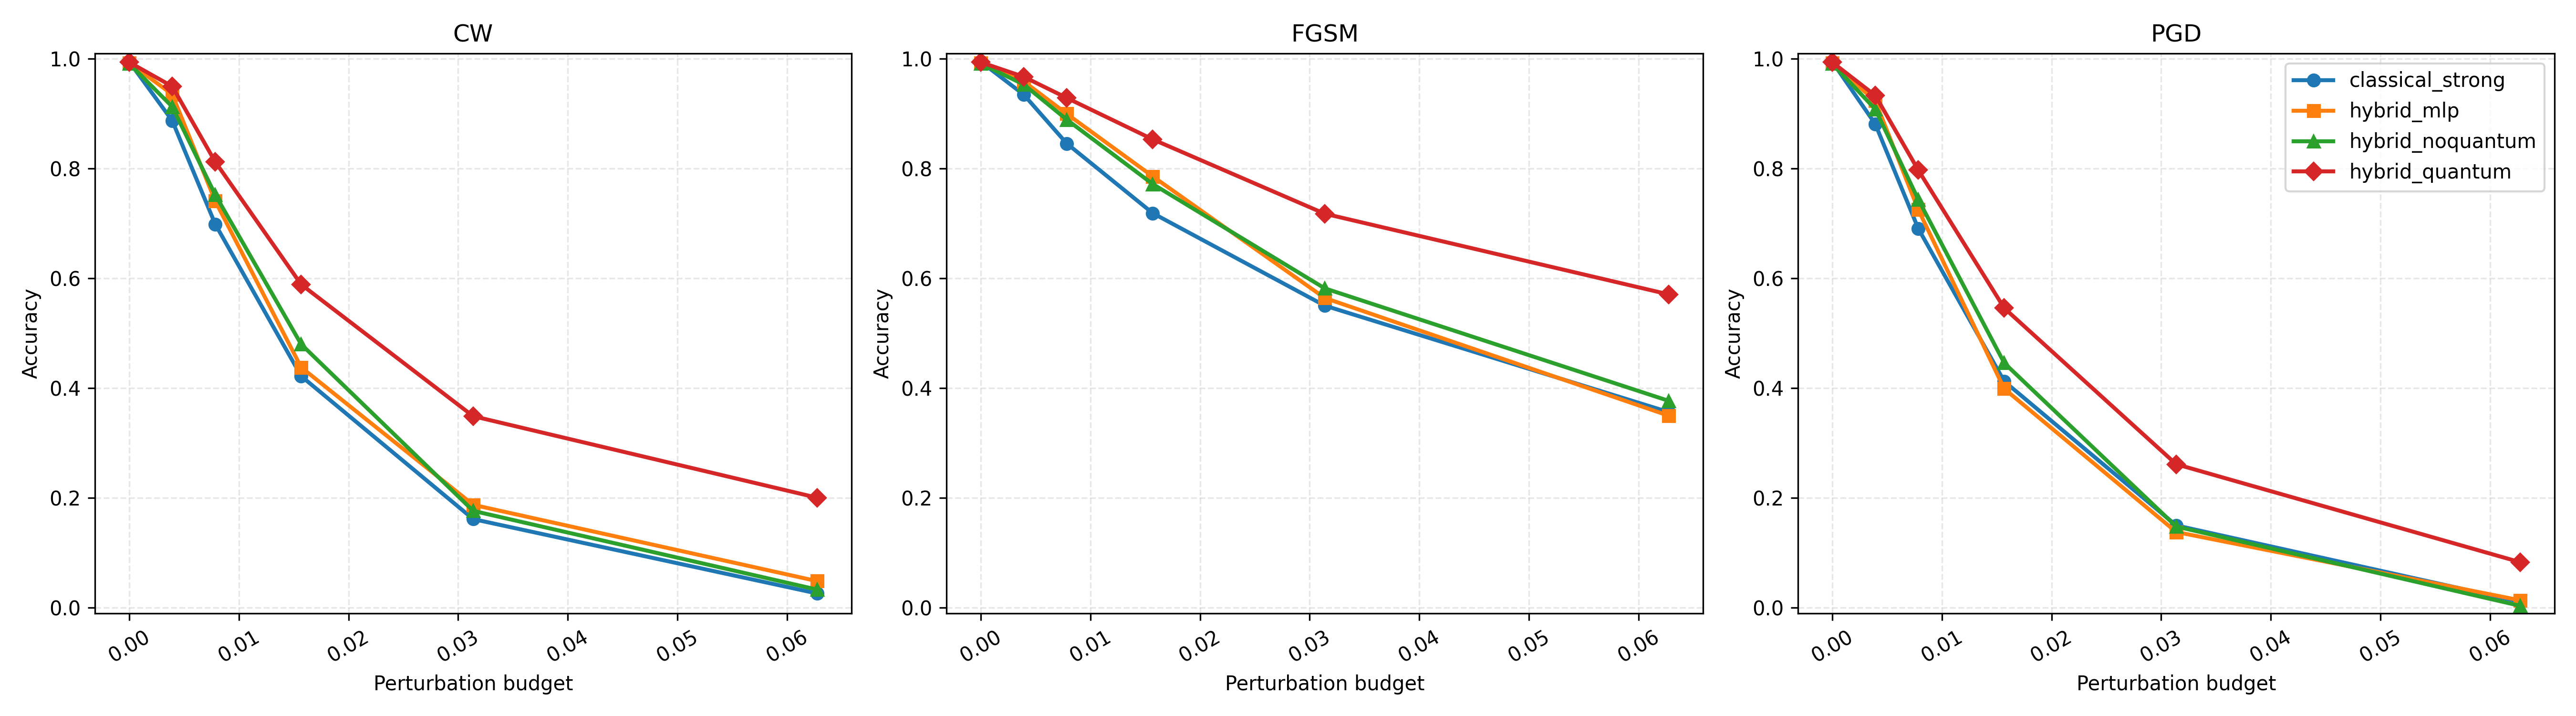
\includegraphics[width=0.95\textwidth]{figures/summary_robustness.png}
\caption{Robust accuracy versus perturbation budget $\eps$ for the four
models under FGSM, PGD, and C\&W attacks. The hybrid quantum model
(\texttt{hybrid\_quantum}, red) retains higher accuracy than the strong
classical baseline and both ablations across nearly all budgets and
attacks.}
\label{fig:robustness}
\end{figure}

\begin{table}[t]
\centering
\caption{Robust accuracy (\%) on GTSRB under FGSM, PGD, and C\&W attacks
at selected perturbation budgets (seed 42, $n=1$). The hybrid quantum
model outperforms the strong classical baseline and both ablations at
every non-trivial budget.}
\label{tab:robust}
\begin{tabular}{llccccc}
\toprule
Attack & Model & $\frac{1}{255}$ & $\frac{2}{255}$ & $\frac{4}{255}$ & $\frac{8}{255}$ & $\frac{16}{255}$ \\
\midrule
\multirow{4}{*}{FGSM}
 & \texttt{classical\_strong} & 93.50 & 84.60 & 71.90 & 55.05 & 35.65 \\
 & \texttt{hybrid\_noquantum} & 95.35 & 88.95 & 77.20 & 58.20 & 37.70 \\
 & \texttt{hybrid\_mlp}        & 95.90 & 90.00 & 78.60 & 56.45 & 35.00 \\
 & \texttt{hybrid\_quantum}    & \textbf{96.75} & \textbf{92.90} & \textbf{85.35} & \textbf{71.80} & \textbf{57.10} \\
\midrule
\multirow{4}{*}{PGD}
 & \texttt{classical\_strong} & 88.15 & 69.10 & 41.25 & 15.00 & 1.10 \\
 & \texttt{hybrid\_noquantum} & 90.85 & 74.40 & 44.60 & 14.80 & 0.35 \\
 & \texttt{hybrid\_mlp}        & 92.35 & 72.55 & 39.90 & 13.80 & 1.35 \\
 & \texttt{hybrid\_quantum}    & \textbf{93.35} & \textbf{79.75} & \textbf{54.60} & \textbf{26.15} & \textbf{8.30} \\
\midrule
\multirow{4}{*}{C\&W}
 & \texttt{classical\_strong} & 88.75 & 69.90 & 42.20 & 16.15 & 2.60 \\
 & \texttt{hybrid\_noquantum} & 91.30 & 75.25 & 48.00 & 17.65 & 3.30 \\
 & \texttt{hybrid\_mlp}        & 93.55 & 74.10 & 43.80 & 18.75 & 4.85 \\
 & \texttt{hybrid\_quantum}    & \textbf{95.00} & \textbf{81.25} & \textbf{58.90} & \textbf{34.90} & \textbf{20.05} \\
\bottomrule
\end{tabular}
\end{table}

The pattern is consistent across attacks and budgets. At the
commonly-reported budget $\eps = 8/255$, \texttt{hybrid\_quantum} retains
$26.15\%$ accuracy under PGD versus $15.00\%$ for
\texttt{classical\_strong}---a relative improvement of roughly $74\%$.
The gap widens further under C\&W ($34.90\%$ vs.\ $16.15\%$) and is also
present, though smaller in absolute terms, under the weaker single-step
FGSM ($71.80\%$ vs.\ $55.05\%$). At the largest budget
$\eps = 16/255$, where all models have degraded substantially, the hybrid
quantum model still outperforms the baseline by more than $21$ points
under FGSM and by $17$ points under C\&W.

%---------------------------------------------------------------------
\subsection{Ablation: Isolating the Quantum Contribution}
\label{sec:exp:ablation}

The robustness gain could, in principle, arise from any of the three
differences between \texttt{hybrid\_quantum} and
\texttt{classical\_strong}: the 8-d bottleneck, the additional nonlinear
head, or the quantum circuit. \Cref{tab:ablation} reports the robust
accuracy of the two ablations alongside the baseline and full hybrid at
$\eps = 8/255$, and \Cref{tab:ablation_delta} reports the accuracy gap
of each model relative to \texttt{classical\_strong}.

\begin{table}[t]
\centering
\caption{Robust accuracy (\%) at $\eps = 8/255$ (seed 42). The two
ablations (\texttt{noquantum}, \texttt{mlp}) recover the classical
baseline's behavior; only \texttt{hybrid\_quantum} shows a gain.}
\label{tab:ablation}
\begin{tabular}{lccc}
\toprule
Model & FGSM & PGD & C\&W \\
\midrule
\texttt{classical\_strong}    & 35.65 & 15.00 & 16.15 \\
\texttt{hybrid\_noquantum}    & 37.70 & 14.80 & 17.65 \\
\texttt{hybrid\_mlp}           & 35.00 & 13.80 & 18.75 \\
\texttt{hybrid\_quantum}       & \textbf{57.10} & \textbf{26.15} & \textbf{34.90} \\
\bottomrule
\end{tabular}
\end{table}

\begin{table}[t]
\centering
\caption{Robust accuracy gap ($\Delta$, percentage points) relative to
\texttt{classical\_strong} at $\eps = 8/255$. The gain is concentrated in
\texttt{hybrid\_quantum}; both ablations are within $\pm 3$ points of the
baseline.}
\label{tab:ablation_delta}
\begin{tabular}{lccc}
\toprule
Model & $\Delta$FGSM & $\Delta$PGD & $\Delta$C\&W \\
\midrule
\texttt{hybrid\_noquantum}    & $+2.05$  & $-0.20$  & $+1.50$ \\
\texttt{hybrid\_mlp}           & $-0.65$  & $-1.20$  & $+2.60$ \\
\texttt{hybrid\_quantum}       & $+21.45$ & $+11.15$ & $+18.75$ \\
\bottomrule
\end{tabular}
\end{table}

The result directly answers \textbf{RQ2}. \texttt{hybrid\_noquantum}
retains the 8-d bottleneck and the $2\pi$ input scaling but removes the
quantum circuit; its robust accuracy at $\eps=8/255$ is within
$2.6$ points of the strong classical baseline under all three attacks.
\texttt{hybrid\_mlp} replaces the quantum circuit with a classical MLP of
comparable depth; it likewise stays within $2.6$ points of the baseline.
Only \texttt{hybrid\_quantum}---the variant that actually executes the
variational quantum circuit---exhibits the robustness gain, and it does
so by $11$--$21$ percentage points depending on the attack.

This rules out the two confounds. The 8-d bottleneck alone does not
confer robustness (\texttt{hybrid\_noquantum} disproves it), and adding
a classical nonlinear head of similar shape does not either
(\texttt{hybrid\_mlp} disproves it). The effect is specific to the
quantum circuit, which we take as evidence that the variational quantum
feature map alters the model's decision geometry in a way that the
gradient-based attackers we evaluate find harder to exploit.

%======================================================================
\section{Discussion and Limitations}
\label{sec:discussion}
%======================================================================

%---------------------------------------------------------------------
\subsection{Why Might the Quantum Layer Improve Robustness?}
\label{sec:disc:mechanism}

We emphasize at the outset that the following discussion is speculative;
pinning down the precise mechanism requires controlled gradient-landscape
and decision-boundary analyses that are beyond the scope of this paper.
Nonetheless, the consistency of the effect across three structurally
distinct attacks (FGSM, PGD, C\&W) and across a wide range of $\eps$ makes
it unlikely to be an artifact of a single attack's failure mode.

A variational quantum circuit is not just another nonlinear layer. Its
input--output map is defined by quantum interference over a Hilbert space
that has no straightforward classical analogue, and the measurement
expectation values depend on the circuit parameters through trigonometric
functions of the inputs and weights. Two qualitative observations may be
relevant.

First, the quantum feature map reshapes the decision geometry. Because
the 8 Pauli-$Z$ readouts live in $[-1,1]$ and are a non-trivial,
periodic function of the 8-d bottleneck, the linear classifier on top
operates in a feature space whose geometry differs from the raw
bottleneck. First-order attackers that exploit the gradient of the loss
with respect to the pixel input may find that the effective gradient
direction---chained through the quantum map---is less aligned with the
true decision boundary than it is for a purely classical head.

Second, gradient-based attacks rely on a locally consistent gradient
signal. The trigonometric dependence of the quantum circuit's output on
its inputs can flatten or oscillate the loss landscape in input space,
so that a single sign-of-gradient step (FGSM) or even a projected
multi-step trajectory (PGD) may converge to a less effective perturbation
than it does for a classical head whose gradient is smoother. The fact
that the gain is largest under C\&W---the strongest of the three attacks
and the one that does not rely on sign-of-gradient steps---suggests the
effect is not merely a gradient-masking artifact in the narrow sense, though
a subtler optimization-landscape effect cannot be ruled out.

%---------------------------------------------------------------------
\subsection{Cross-Attack Consistency}
\label{sec:disc:consistency}

A natural concern with any reported robustness gain is whether it reflects
a genuine property of the model or a weakness of the specific attack
used to probe it~\cite{tramer2020adaptive}. We mitigate this by
reporting three attacks of fundamentally different character: FGSM is a
single-step, sign-based attack; PGD is a multi-step, sign-based attack
with random restarts; and C\&W is a continuous-optimization attack with
an Adam solver and a margin-based loss. The hybrid quantum model
outperforms the strong classical baseline under all three, and the
ablations fail to reproduce the gain under all three. This
cross-attack consistency is evidence that the effect is a property of the
model rather than of any one attack's failure mode.

%---------------------------------------------------------------------
\subsection{Limitations}
\label{sec:disc:limits}

We are explicit about the boundaries of what our study establishes.

\paragraph{Single seed.}
All results are reported for a single random seed ($42$), so $n=1$ and
no standard errors are available. The pattern is consistent across three
attacks, five non-trivial perturbation budgets, and two non-trivial
ablations, which makes a chance result less likely, but multi-seed
evaluation is necessary before drawing strong conclusions. We flag this
as the most important follow-up.

\paragraph{Simulated quantum hardware.}
The variational circuit is simulated on PennyLane's
\texttt{default.qubit} device. Real quantum hardware introduces gate
noise, finite sampling, and connectivity constraints that may alter the
learned feature map and hence the robustness behavior. Our results
characterize the \emph{ideal-circuit} regime.

\paragraph{Digital white-box attacks only.}
We do not evaluate physical attacks (RP2-style patches, EOT-transformed
perturbations) that are central to the autonomous-driving threat model.
The robustness gain we observe is under digital white-box attacks;
transferring it to the physical world is an open question.

\paragraph{Input resolution.}
GTSRB images are resized to $32\times32$, which is lower than some
prior robustness work on this benchmark. This matches the WideResNet
input convention and keeps the quantum simulation tractable, but it
discards fine-grained sign detail that higher-resolution inputs would
preserve.

\paragraph{No adaptive-attack evaluation.}
A reviewer could argue that the quantum layer acts as a gradient mask
and that an adaptive attack designed with the quantum layer's
differentiability in mind would close the gap. Our C\&W results partially
address this (it is a continuous optimizer, not a sign-of-gradient
attack), but a dedicated adaptive-attack study~\cite{tramer2020adaptive}
is needed for a definitive claim.

%======================================================================
\section{Conclusion}
\label{sec:conclusion}
%======================================================================

We presented, to our knowledge, the first adversarial robustness
evaluation of a quantum-classical hybrid model on a safety-critical
autonomous driving task. On GTSRB, a hybrid WideResNet with an 8-qubit,
6-layer variational quantum circuit is compared against a strong
classical WideResNet baseline and two structural ablations, all sharing
an identical backbone and achieving clean accuracy within a 0.7-point
band. Under white-box FGSM, PGD, and C\&W attacks, the hybrid quantum
model consistently retains higher robust accuracy---at $\eps=8/255$
under PGD, $26.15\%$ versus $15.00\%$ for the strong baseline.

A controlled ablation isolates this gain to the quantum layer itself:
removing the quantum circuit or replacing it with a classical MLP both
erase the effect, while preserving the 8-dimensional bottleneck and the
additional nonlinearity. This rules out the two most obvious confounds
and attributes the robustness difference to the quantum feature map.

Our results are bounded by single-seed evaluation, ideal-circuit
simulation, and digital white-box attacks. Whether the gain survives
multi-seed evaluation, real quantum noise, and physical attacks remains
open. If it does, quantum-augmented classifiers may offer a
complementary axis of robustness for safety-critical perception; if it
does not, the negative result itself would clarify the limits of quantum
machine learning in adversarial settings. Either outcome motivates the
next round of experiments we outline as future work: multi-seed
re-evaluation, adaptive-attack evaluation, EOT-based physical attack
transfer, and, ultimately, deployment on near-term quantum hardware.

\bibliographystyle{plain}
\bibliography{references}

\end{document}
